\documentclass[11pt, a4paper]{article}

\usepackage{amsmath}
\usepackage{amsfonts} %Matheschriften
\usepackage{amssymb} %Mathesymbole
%\usepackage{mathptmx} % Einstellung für Schriften und Sonderzeichen in mathematischen Umgebungen
                        % ändert SChriftfont
\usepackage{wasysym} % Stellt diverse Sonderzeichen bereit
\usepackage{siunitx}
\usepackage{float}
\usepackage{microtype}
\usepackage{graphicx}
\usepackage{hyperref}
\usepackage{xcolor}
\usepackage[section]{placeins}
% allows for temporary adjustment of side margins
\usepackage{changepage}
\usepackage{rotating}


% \usepackage[ngerman]{babel}
% \addto\captionsngerman{%
%  \renewcommand{\abstractname}{Einleitung}}

\title{Versuch 4: Transistor}
\author{Team 2-13: Jascha Fricker, Benedict Brouwer}

\begin{document}
    \maketitle

    \tableofcontents

    \newpage
\section{Introduction}
In this experiment we examine the properties of a bipolar transistor as a class A amplifier. To observe the proporties we measured the characteristic curve 
of the transistor and tested different configurations of the emitter circuit.
\section{Theorie}

\FloatBarrier
\subsection{Small Signal Model}
For small deviations around the operating point one can use the small signal modell leading to the following equation.
\begin{align}
\left(\begin{array}{l}
    d I_{\mathrm{B}} \\
    d I_{\mathrm{C}}
    \end{array}\right)=\left(\begin{array}{cc}
    \frac{1}{r_{\mathrm{BE}}} & S_{\mathrm{r}} \\
    S & \frac{1}{r_{\mathrm{CE}}}
    \end{array}\right)\left(\begin{array}{l}
    d U_{\mathrm{BE}} \\
    d U_{\mathrm{CE}}
    \end{array}\right)
    \label{eq:ssm}
\end{align}

whereby $r_{\text{BE}}$, $r_{\text{CE}}$ and the steepness $S$ can be calculated with
\begin{align}
    \frac{1}{r_{\text{BE}}} = \frac{\partial I_{\text{B}}}{\partial U_{\text{BE}}} |_{U_{\text{CE}}} \label{eq:rbe} 
\end{align}
\begin{align}
    \frac{1}{r_{\text{CE}}} = \frac{\partial I_{\text{C}}}{\partial U_{\text{CE}}} |_{U_{\text{BE}}} \label{eq:rce} 
\end{align}
\begin{align}
    S=\left .\frac{\partial I_{\mathrm{C}}}{\partial U_{\mathrm{BE}}}\right |_{U_{\mathrm{CE}}}=\frac{q I_{\mathrm{C}}}{k_{\mathrm{B}} T} \label{eq:steep}
\end{align}

In addition to that $I_{\mathrm{B}}$ can be calculated the following proportionality 
\begin{align}
    I_{\mathrm{B}} \propto \exp \left(\frac{q U_{\mathrm{BE}}}{k_{\mathrm{B}} T}\right)
    \label{eq:Ib_T}
\end{align}

\FloatBarrier
\subsection{Emitter Circuit}
An emitter circuit converts an input sigal to an amplified output signal. The amplification of the output signal compared to the input signal can is given by


\begin{align}
    A=\frac{d U_{\mathrm{a}}}{d U_{\mathrm{e}}}=-S \cdot\left(R_{\mathrm{C}}\left\|r_{\mathrm{CE}}\right\| R_{\mathrm{L}}\right)
    \label{eq:ampEasy}
\end{align}
and 
\begin{align}
A \approx-\frac{R_{\mathrm{C}} \| R_{\mathrm{L}}}{R_{\mathrm{E}}}
\label{eq:ampDrift}
\end{align}
if the amplification is in the range of basevoltage drift.
\section{Execution}
\begin{figure}[h]
    \centering
    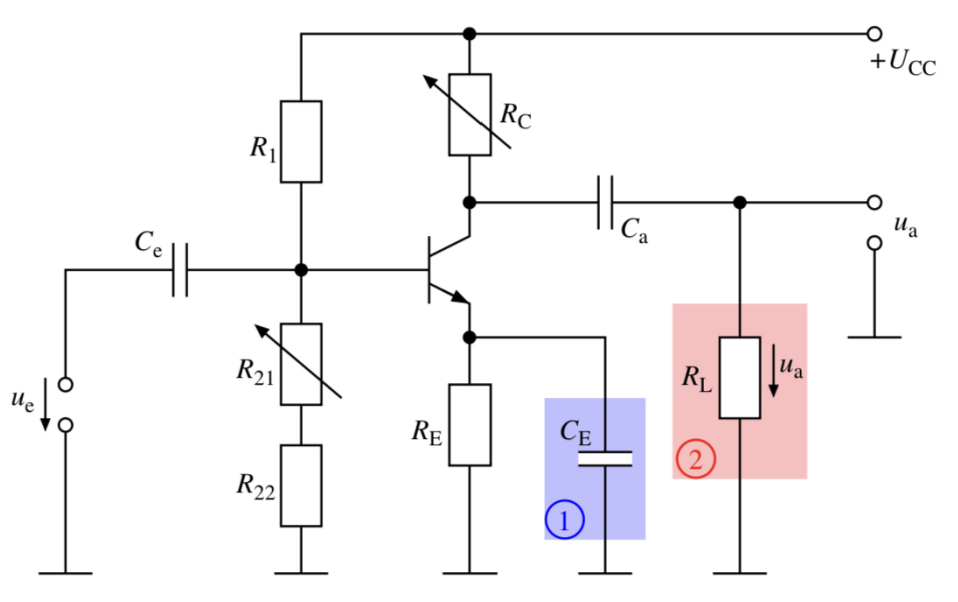
\includegraphics[width=0.8\textwidth]{bilder/Emitter circuit.png}
    \caption{emittercircuit:\\
    $R_1$ = 47 \si{\kilo\ohm}, $R_{22}$ = 100 \si{\ohm},$R_E$ = 10 \si{\kilo\ohm}, $C_e$ = 47 \si{\micro\farad},$C_a$ = 470 \si{\micro\farad}, $U_{CC}$ = 9 \si{\volt} 
    $R_{12}$: potentiometer for the operating point, $R_C$: potentiometer 0 - 10 \si{\kilo\ohm}, $u_e$: inputvoltage, $u_a$: outputvoltage
    }
    \label{im:Emcir}
\end{figure}

\FloatBarrier
\subsection{Operating Point}
A bipolar transistor has a specific basevoltage range (the so called operating point) in which it behaves approximately linear. This operating point
is tuned by setting the resistance at the potentiometer $R_{12}$ (see circuit diagram \ref{im:Emcir}) to a point whereby the output amplitude $u_a$ is maximal and the signal is not distorted.
To tune the operating point, the load resistor $R_L$ was removed and a sinusoidal frequency of 5.5 \si{\kilo\hertz} was applied. 
$U_{\text{BE}}$, $U_{\text{CE}}$, $I_{\text{C}}$ where measured with varying $R_{\text{C}}$ for further evaluation.
\FloatBarrier
\subsection{Amplification of the Emittercircuit}
To further examine the emitter circuit(see circuit diagram  \ref{im:Emcir}) the amplitude ratio $u_a / u_e$ was measured for varying $R_{\text{C}}$ in different circuit configurations:\\
1. with capacitor $C{\text{E}}$ but without resistor $R_{\text{L}}$
2. without capacitor $C{\text{E}}$ and without resistor $R_{\text{L}}$
3. with capacitor $C{\text{E}}$ and resistor $R_{\text{L}}$
\FloatBarrier
\subsection{Frequency Response}
In this experiment the input frequency was varied from 6 \si{\hertz} - 250 \si{\kilo\hertz} to measure the phase shift and the amplidude ratio $u_a / u_e$. 
Here circuit \ref{im:Emcir} with an collector resistor of $R_{\text{C}}$ was used. In addition to that the oszilloscope was changed to x-y mode to observe lissajous curves.
\FloatBarrier
\subsection{Characteristic Curve}
\begin{figure}[h]
    \centering
    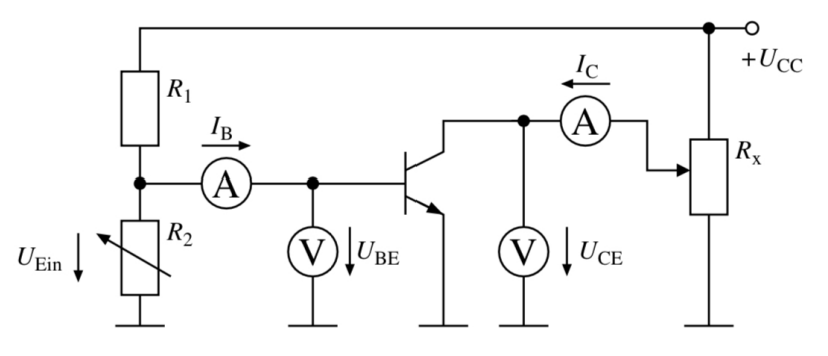
\includegraphics[width=0.8\textwidth]{bilder/characteristicCurve.png}
    \caption{characteristic curve \\
    $R_1$ = 1 \si{\kilo\ohm}, $R_2$ = 220 \si{\ohm}}
    \label{im:Charcurcir}
\end{figure}

To measure the characteristic curve of the transistor the circuit was change as shown in the circuit diagram \ref{im:Charcurcir}. 
First the entry curve $I_{\text{B}}=f(U_{\text{BE}})|_{U_{\text{CE}}}$ was taken by changing $U_{\text{BE}}$ from 0 to 670 \si{\milli\volt} and measuring $I_{\text{B}}$,
$U_{\text{BE}}$ and $U_{\text{CE}}$ with multimeters according to the schematic \ref{im:Charcurcir}. Therby $U_{\text{CE}}$ was dialed in to match the results from experiment 1 \ref{tab:operating point_measurement} with $R_{\text{C}}$ = 5 \si{\kilo\ohm}.
Afterwards the output characteristic curve $I_{\text{C}} = f(U_{\text{CE}})|_{U_{\text{BE}}}$ was recorded with a varying $U_{\text{CE}}$ from 1 - 10 \si{\volt} by measuring $I_{\text{C}}$, $U_{\text{BE}}$ and $U_{\text{CE}}$. This curve was measured in both directions to observe the effect of heat on the transistor.

\section{Evaluation and Results}
\FloatBarrier
\subsection{Preliminary Considerations}

\subsubsection{Measuring of the characteristic Values}
The characteristic values of a transistor are different for each operating point. Therefore the measurements have to be done with the voltages already applied. This could messs with the multimeter leadiging to wrong measurements, if it assumes free floating ends. This also means that the resistance of the power supply and the resistor have to be taken into account, as is essentialy a second path for energy to flow parallel. Lastly the test voltage, which the multimeter uses to probe the resistance could be greater than the maximum of the small signal model, so that the multimeter measures outside the linear section. But if you either assume, that the flow of energy through the power supply is negligeble or that the transistor can be measured outside of the circuit, with three measurements each the resistances and capacitances can be calculated with formulas for a delta configuration. The arraangement can be seen in \cite[figure 11]{TRA}.

\subsubsection{Transformation of y to h parameters}
The dependency of $i_1$, $i_2$, $u_1$ and $u_2$ in the small signal model \ref{eq:ssm} can also be written in h parameter form as
\begin{align}
    \begin{pmatrix}
        u_{BE} \\
        i_c
    \end{pmatrix}
    = 
    \begin{pmatrix}
        r_{BE} & 0 \\
        S \cdot r_{BE} & \frac{1}{r_{CE}}
    \end{pmatrix}
    \begin{pmatrix}
        i_b \\
        u_{CE}
    \end{pmatrix} \,.
    \label{eq:mat}
\end{align}
Wih the formulas on the worksheet the small signal amplification $\beta$ can be calculated
\begin{align}
    u_{BE} &= i_b r_{BE} \text{see \ref{eq:mat}}\\
    u_{re} &= \left( 1 + \beta \right) i_b R_E \text{see \cite[figure 8 and formula (24)]{TRA}}\\
    u_e &= i_b r_{BE} + \left( 1 + \beta \right) i_b R_e = i_b r_{BE} + u_{re} \text{see \cite[formula (28)]{TRA}} \\
    S\left( u_e - u_{re} \right) &= \beta i_b = S \left( i_b r_{BE} + u_{re} - u_{re} \right) = S i_b r_{BE} \text{see \cite[formula (27)]{TRA}} \\
    \Rightarrow \quad \beta &= S r_{BE} \,.
\end{align}




\FloatBarrier
\subsection{Characteristic Curve (Assignment 7)}
As shown in table \ref{tab:operating point_measurement} some basevalues were recorded which were needed in following experiments. They seem to be in a reasonable range.

\begin{table}[H]
    \centering
    \begin{tabular}{c|c|c|c|c}
    
        $R_{\text{C}}$ in \si{\kilo\ohm}  & $U_{\text{BE}}$ in \si{\volt} & $U_{\text{CE}}$ in \si{\volt} & $I_{\text{C}}$ in \si{\milli\ampere} & $S$ in \si{1\per\ohm} \\ \hline
        1 & 0,57 & 7,86 & 0,58 & 0.025\\ 
        5 & 0,57 & 5,53 & 0,58 & 0.025\\ 
        10 & 0,57 & 3,22 & 0,58 & 0.025\\ 
    \end{tabular}
    \label{tab:operating point_measurement}
    \caption{Base values}
\end{table}

The characteristic input curve is plotted in figure \ref{fig:Eincur}. With the slope of the tangent one can calculate the base resistance $r_{\text{BE}}$ = 3.92 \si{\kilo\ohm} with equation \ref{eq:rbe}. 
The operating temperature $T$ = 272,2 \si{\kelvin} can be obtained by using the fitparameters from the exponetial fit and equation \ref{eq:Ib_T}. Although the operating temperature has the correct magnitude it should be at least 30 \si{\kelvin} higher.
With this operating temperature and equation \ref{eq:steep} the steepness $S$ can be calculated as shown in figure \ref{tab:operating point_measurement}.

\begin{figure}[h]
    \centering
    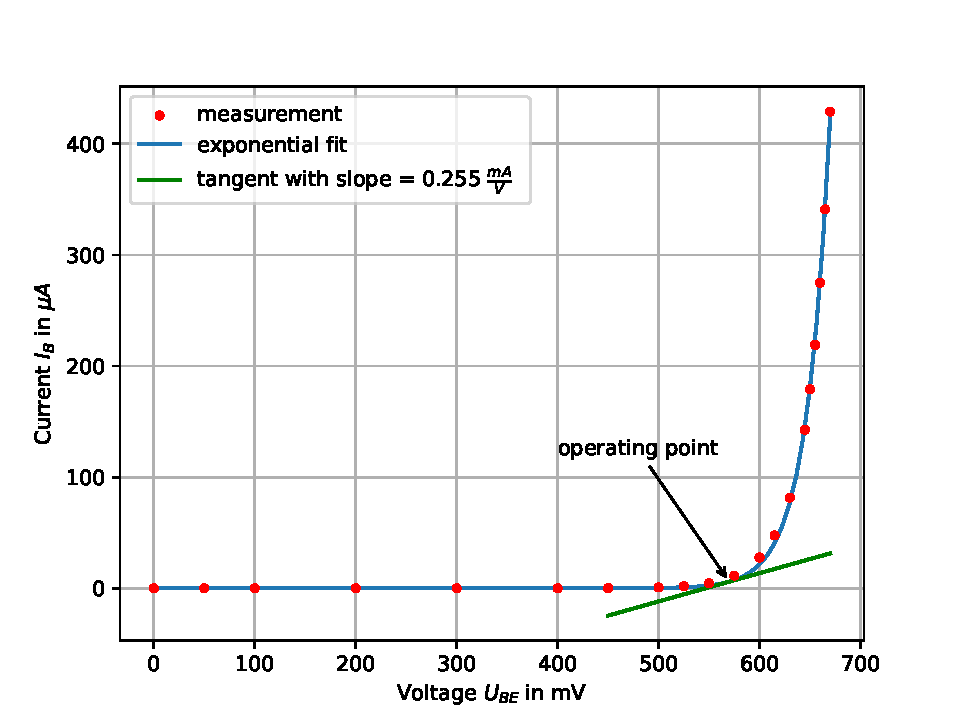
\includegraphics[width=0.8\textwidth]{plots/Eingangskennlinie.pdf}
    \caption{Characteristic curve from the input}
    \label{fig:Eincur}
\end{figure}

\begin{figure}[h]
    \centering
    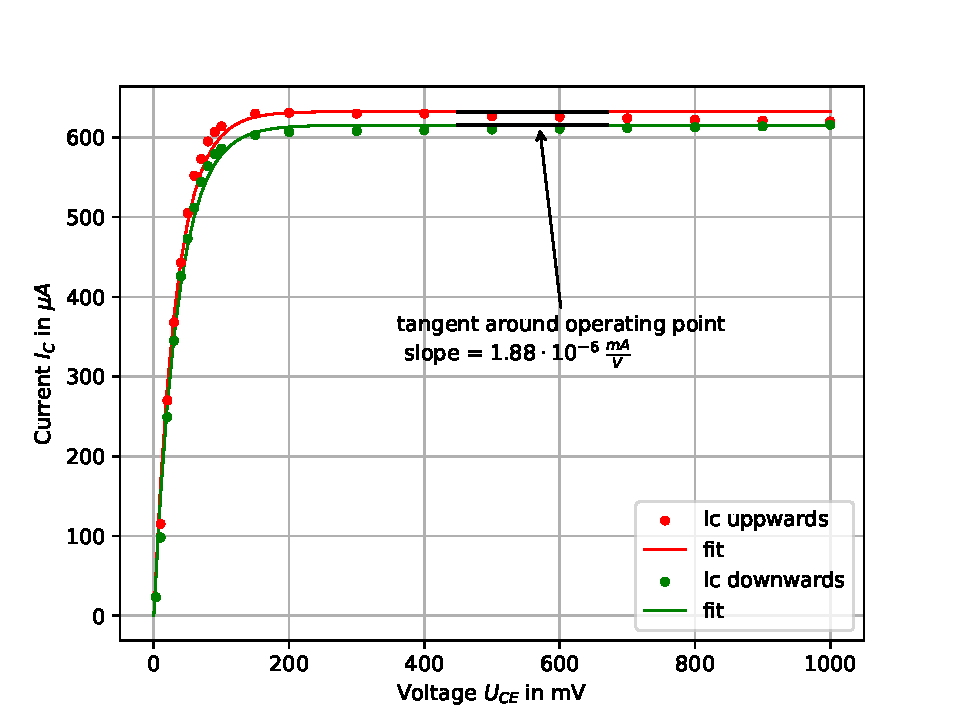
\includegraphics[width=0.8\textwidth]{plots/Ausgangskennlinie.pdf}
    \caption{Characteristic curve from the output}
    \label{fig:Outcur}
\end{figure}
The characteristic output curve is plotted in figure \ref{fig:Outcur}. By utilizing equation \ref{eq:rce} one can calculate the collector - emitter resistance $r_{\text{CE}}$ = 532 \si{\kilo\ohm} with the slope of the tangent.
The high resistance was anticipated because no current should flow from collector to emitter in the closed transistor state.
\FloatBarrier
\subsection{Amplification (Assignment 8)}
\begin{figure}[h]
    \centering
    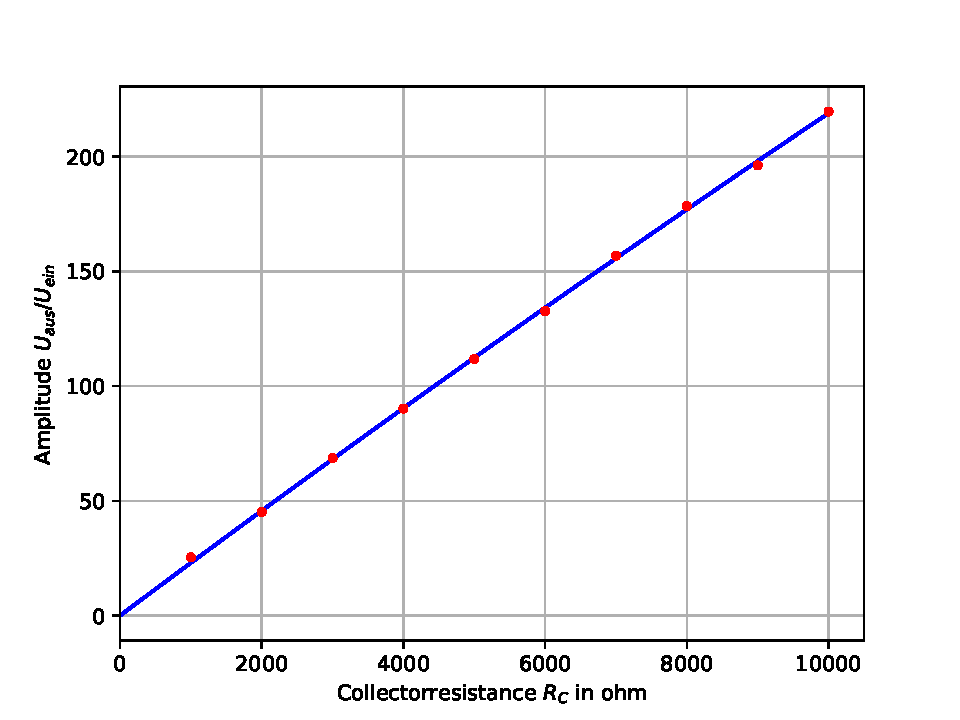
\includegraphics[width=0.8\textwidth]{plots/RC1.pdf}
    \caption{Amplification curve of the emitter circuit with capacitor $C_{\text{E}}$ and without load resistor $R_{\text{L}}$}
    \label{fig:RC1}
\end{figure}

\begin{figure}[h]
    \centering
    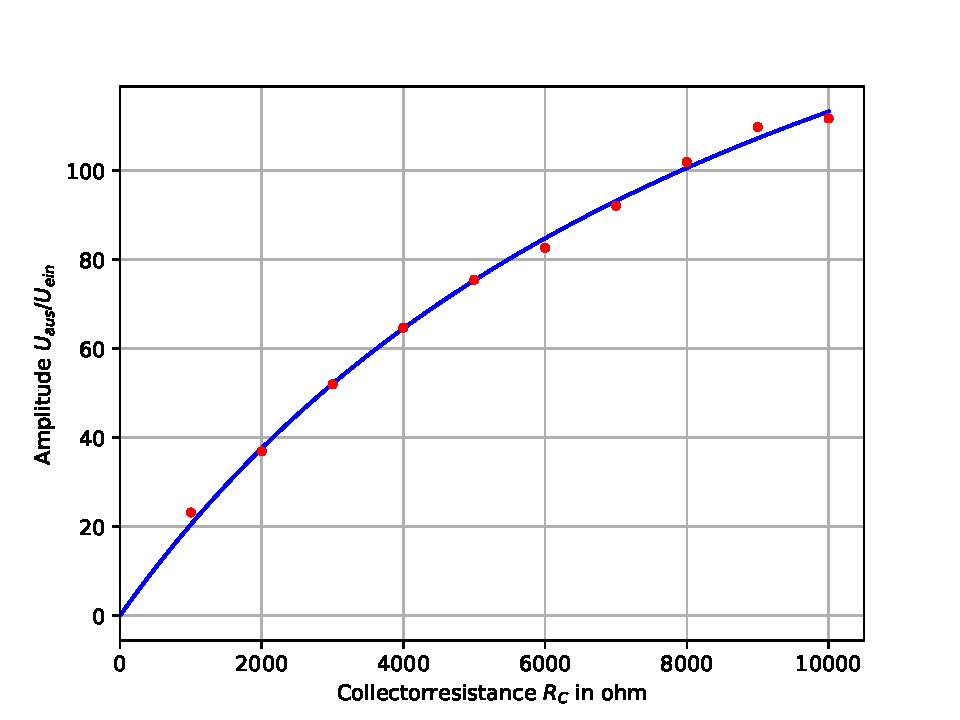
\includegraphics[width=0.8\textwidth]{plots/RC3.pdf}
    \caption{Amplification curve of the emitter circuit with capacitor $C_{\text{E}}$ and load resistor $R_{\text{L}}$}
    \label{fig:RC3}
\end{figure}
The voltage amplification with and without load resistor is shown in figure \ref{fig:RC1} and \ref{fig:RC3}. To calculate the amplification, equation \ref{eq:ampEasy} was used due to the non conductive properties of $C_{\text{E}}$ in low frequency ranges.
While figure \ref{fig:RC1} and \ref{fig:RC2} display a linear behavior, figure \ref{fig:RC3} shows saturating properties.


\begin{figure}[h]
    \centering
    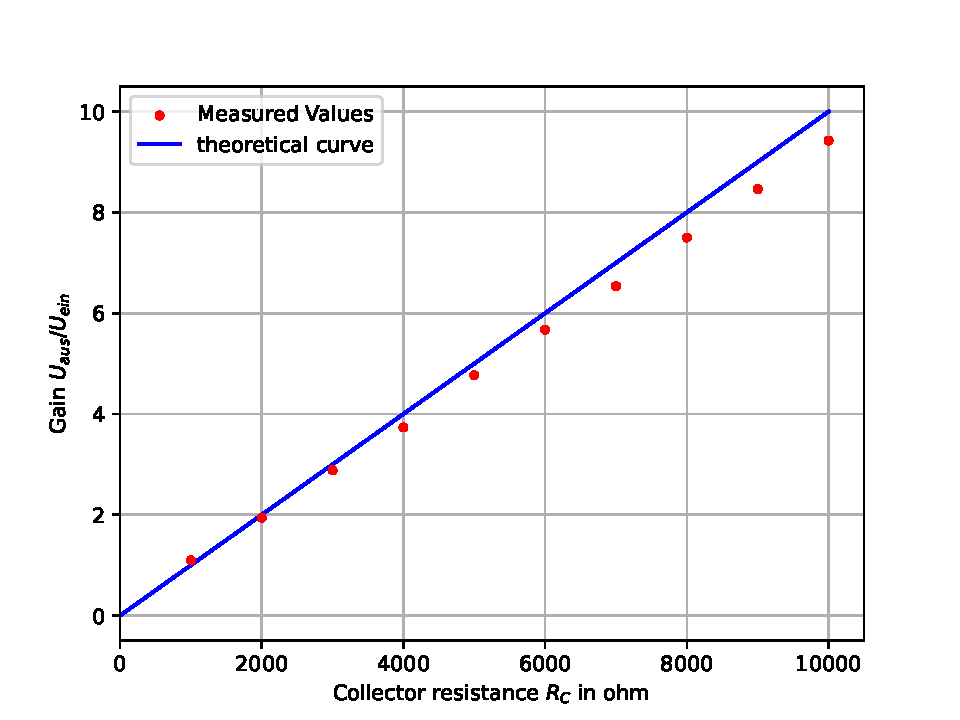
\includegraphics[width=0.8\textwidth]{plots/RC2.pdf}
    \caption{Amplification curve of the emitter circuit without capacitor $C_{\text{E}}$ and load resistor $R_{\text{L}}.$}
    \label{fig:RC2}
\end{figure}
By removing the emitter capacitor $C_{\text{E}}$ the emitter circuit cannot work properly and one can only observe base voltage drift. Therfore we used equation \ref{eq:ampDrift} to fit the measured values as shown in figure \ref{fig:RC2}.
While figure \ref{fig:RC1} and \ref{fig:RC2} display a linear behavior, figure \ref{fig:RC3} shows saturating properties.
The measured values match the calculated curves pretty closely without any outliers.

\FloatBarrier
\subsection{Frequency Response (Assignment 9)}
Another important characteristic of a transistor is the frequency response. Therefore the amplitude and phase response is plotted in figure \ref{fig:Ampresp} and \ref{fig:Pharesp}.
Therby the amplidude response behaves like a high pass filter from 0 - $10^3$ \si{\hertz} and like a low pass filter from $10^3$ - $10^6$ \si{\hertz}.
The section of frequencies, where $\left\lvert A \right\rvert \geq \frac{1}{\sqrt{2}}  \cdot \left\lvert A_{max} \right\lvert$ is also shown in figure \ref{fig:Ampresp}


\begin{figure}[h]
    \centering
    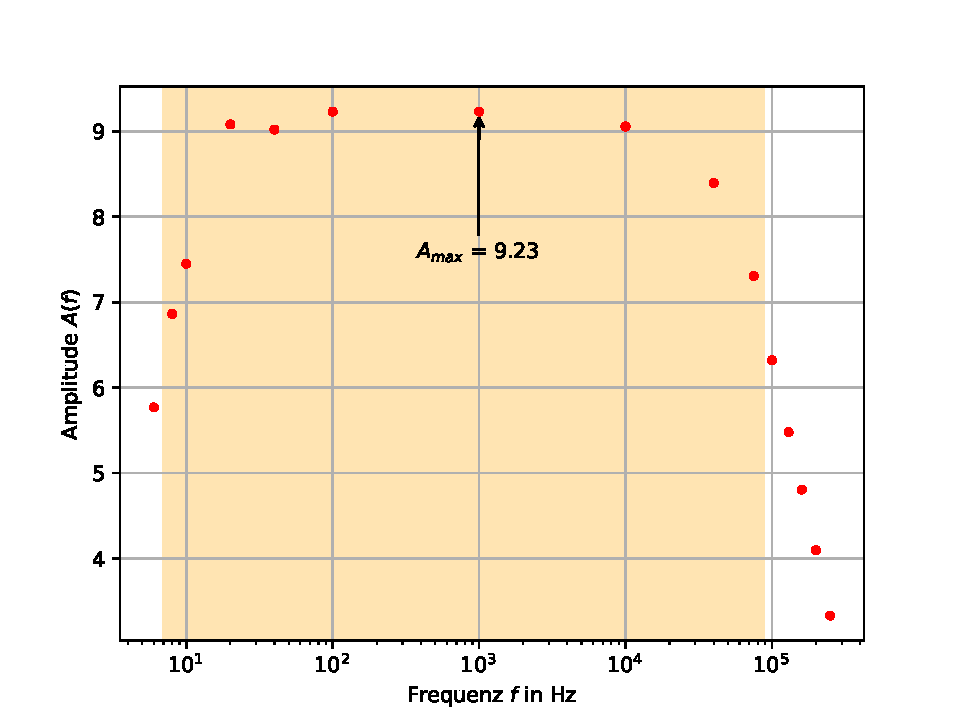
\includegraphics[width=0.8\textwidth]{plots/Amplitudengang.pdf}
    \caption{Amplitude response for different frequencies}
    \label{fig:Ampresp}
\end{figure}

\begin{figure}[h]
    \centering
    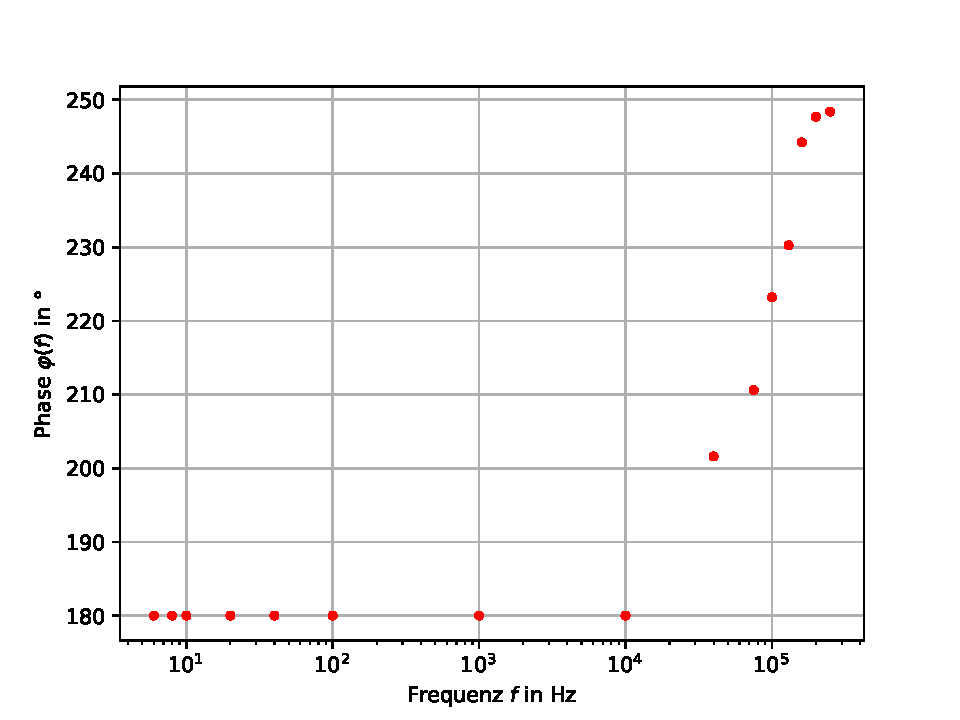
\includegraphics[width=0.8\textwidth]{plots/Phasengang.pdf}
    \caption{Phase response for different frequencies}
    \label{fig:Pharesp}
\end{figure}

\FloatBarrier
\subsection{Transfer Function}
The transfer function $H$ of the schematic in \cite[figure 5]{TRA}, two complex resistors in serial, can be calculate with Kirchhoff's laws
\begin{align}
    H\left(Z_1, Z_2\right) = \frac{U_A}{U_E} = \frac{Z_2}{Z_1 + Z_2} \,.
\end{align}
It is assumed that $I_A = 0$.
If $Z_1 = \frac{1}{i \omega C}$ is a capacitor and $Z_2 = R$ is a resistor, the function can be simplified to
\begin{align}
    H\left( \omega \right) = \frac{R}{R + \frac{1}{i \omega C}}\,.
\end{align}
This is a high pass filter, because if $\omega$ gets bigger, the denominator gets smaller and $H$ gets bigger. So high frequencies are attenuated less than low frequencies

If $Z_1 = $ is a resistor and $Z_2  = \frac{1}{i \omega C}$ is a capacitor, the function can be simplified to
\begin{align}
    H\left(\omega\right) = \frac{\frac{1}{i \omega C}}{R + \frac{1}{i \omega C}} = \frac{1}{1 + i \omega C R} \,.
\end{align}
This circuit is a low pass filter, because if $\omega$ gets bigger, $H$ gets smaller. Low frequencies can pass with less loss than high frequencies.

\bibliographystyle{plain}
\bibliography{literature}

\end{document}

